\subsubsection{Attitude Controller Simulation}

Final Response:

\begin{figure}[H]
	\centering
	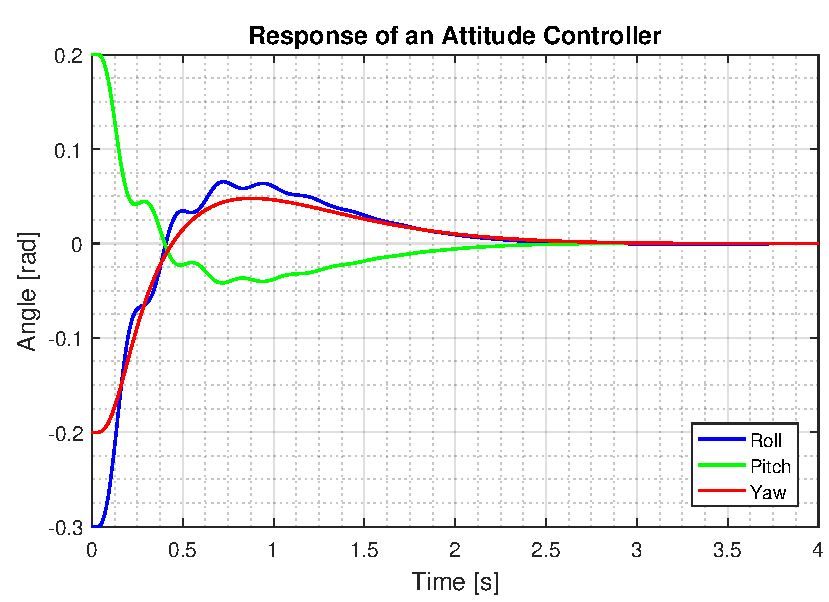
\includegraphics[scale=0.8]{figures/ssFinalEq.pdf}
	\caption{ \autoref{app:matricesSS}.}
	\label{fig:TranslationalControlDiagram}
\end{figure}

%\begin{figure}[H]
%	\centering
%	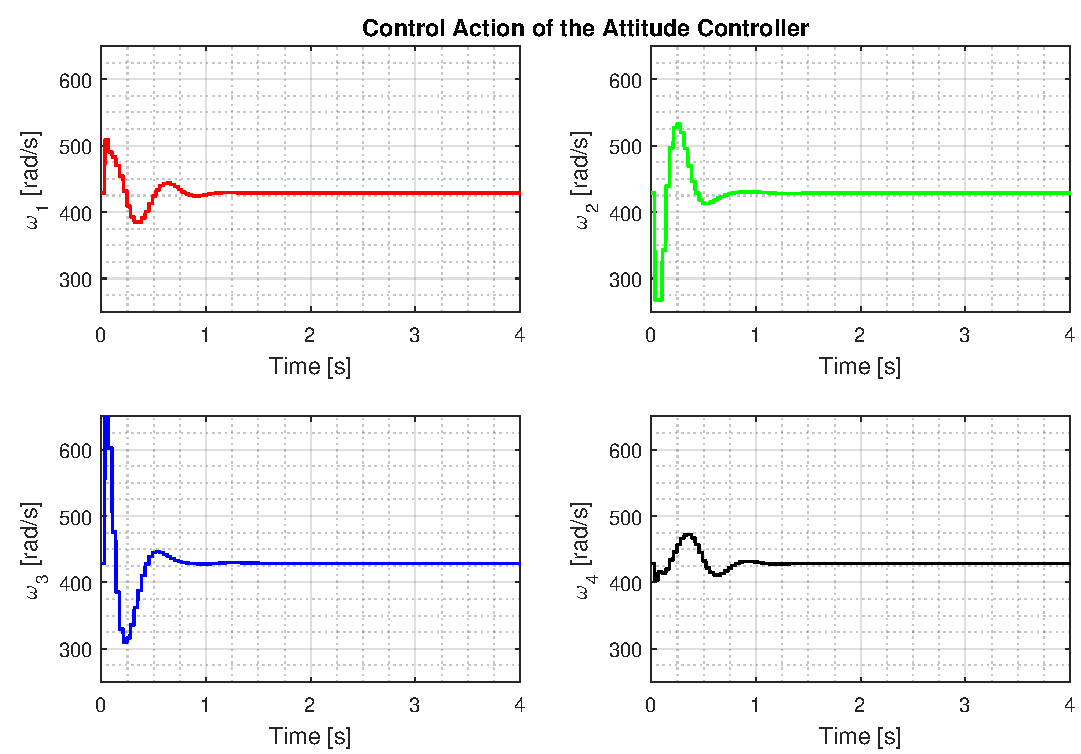
\includegraphics[scale=0.8]{figures/ssFinalEqAction.pdf}
%	\caption{.}
%	\label{fig:TranslationalControlDiagram}
%\end{figure}

Final step response:

\begin{figure}[H]
	\centering
	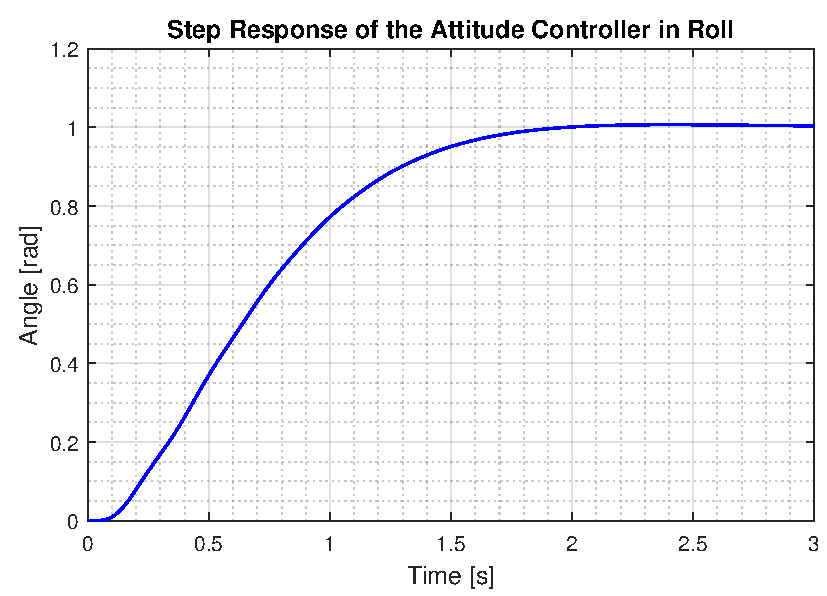
\includegraphics[scale=0.8]{figures/ssFinalStep.pdf}
	\caption{\autoref{app:matricesSS}.}
	\label{fig:TranslationalControlDiagram}
\end{figure}

%\begin{figure}[H]
%	\centering
%	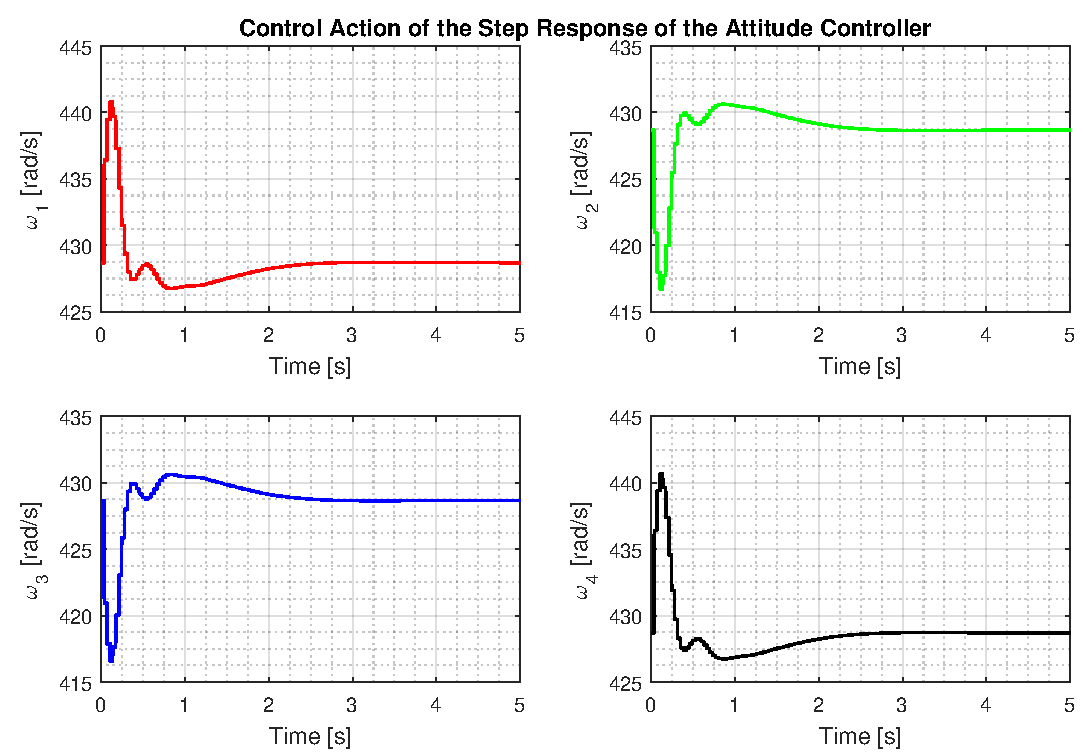
\includegraphics[scale=0.8]{figures/ssFinalStepAction.pdf}
%	\caption{.}
%	\label{fig:TranslationalControlDiagram}
%\end{figure}

Higher F gain:

\begin{figure}[H]
	\centering
	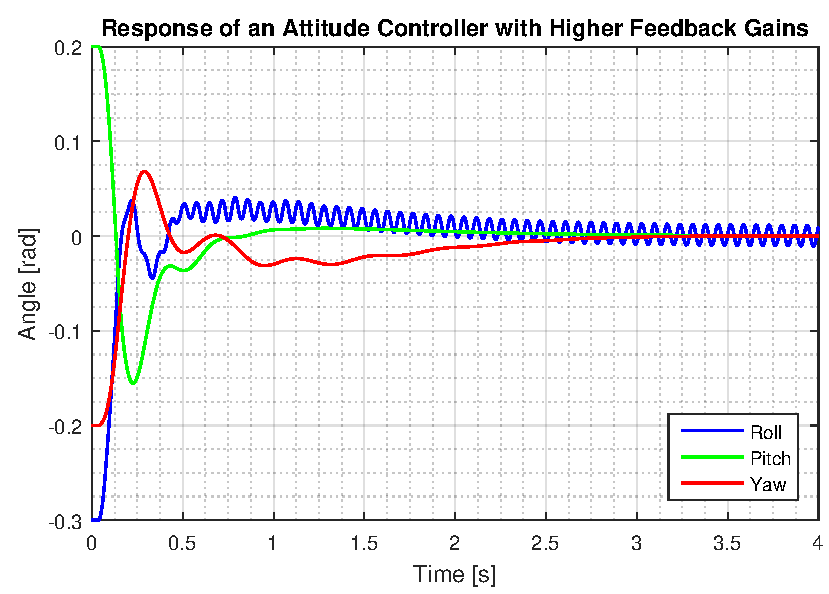
\includegraphics[scale=1]{figures/ssEqBad.pdf}
	\caption{\autoref{app:matricesSS}.}
	\label{fig:TranslationalControlDiagram}
\end{figure}

\begin{figure}[H]
	\centering
	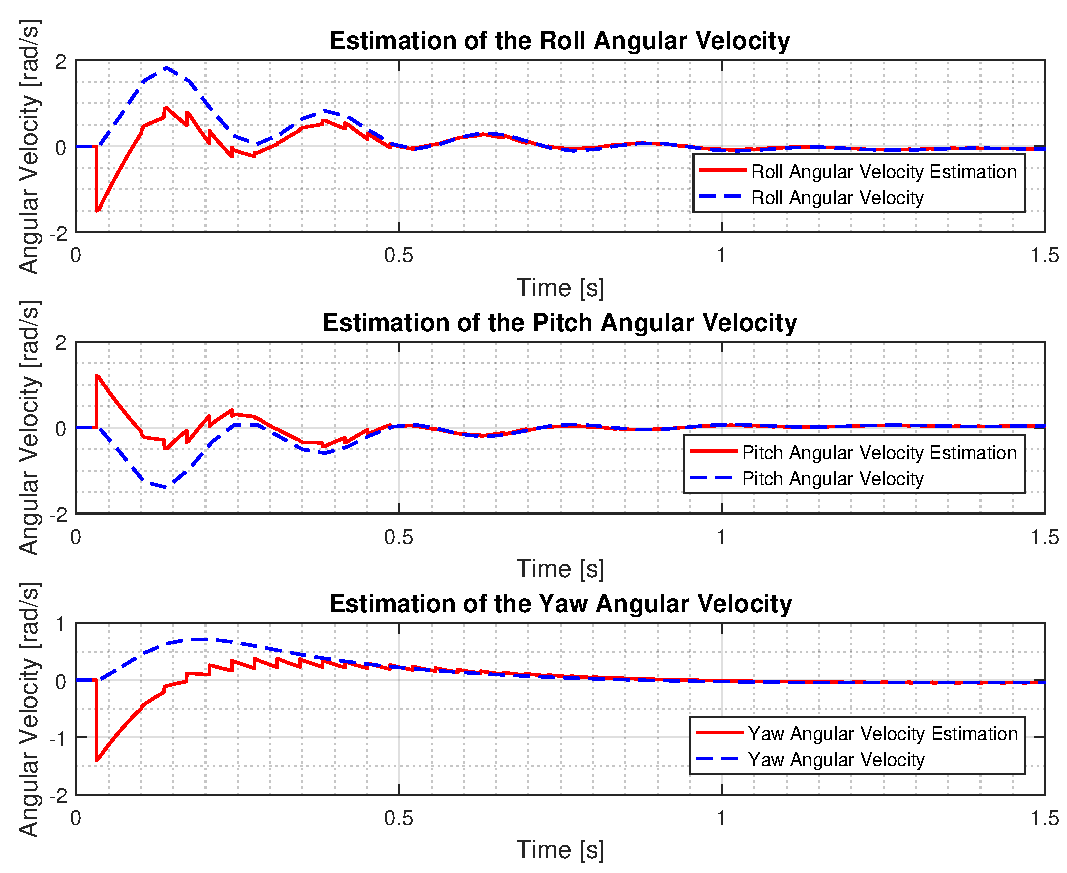
\includegraphics[scale=1]{figures/ssObsFinal.pdf}
	\caption{\autoref{app:matricesSS}.}
	\label{fig:TranslationalControlDiagram}
\end{figure}

\begin{figure}[H]
	\centering
	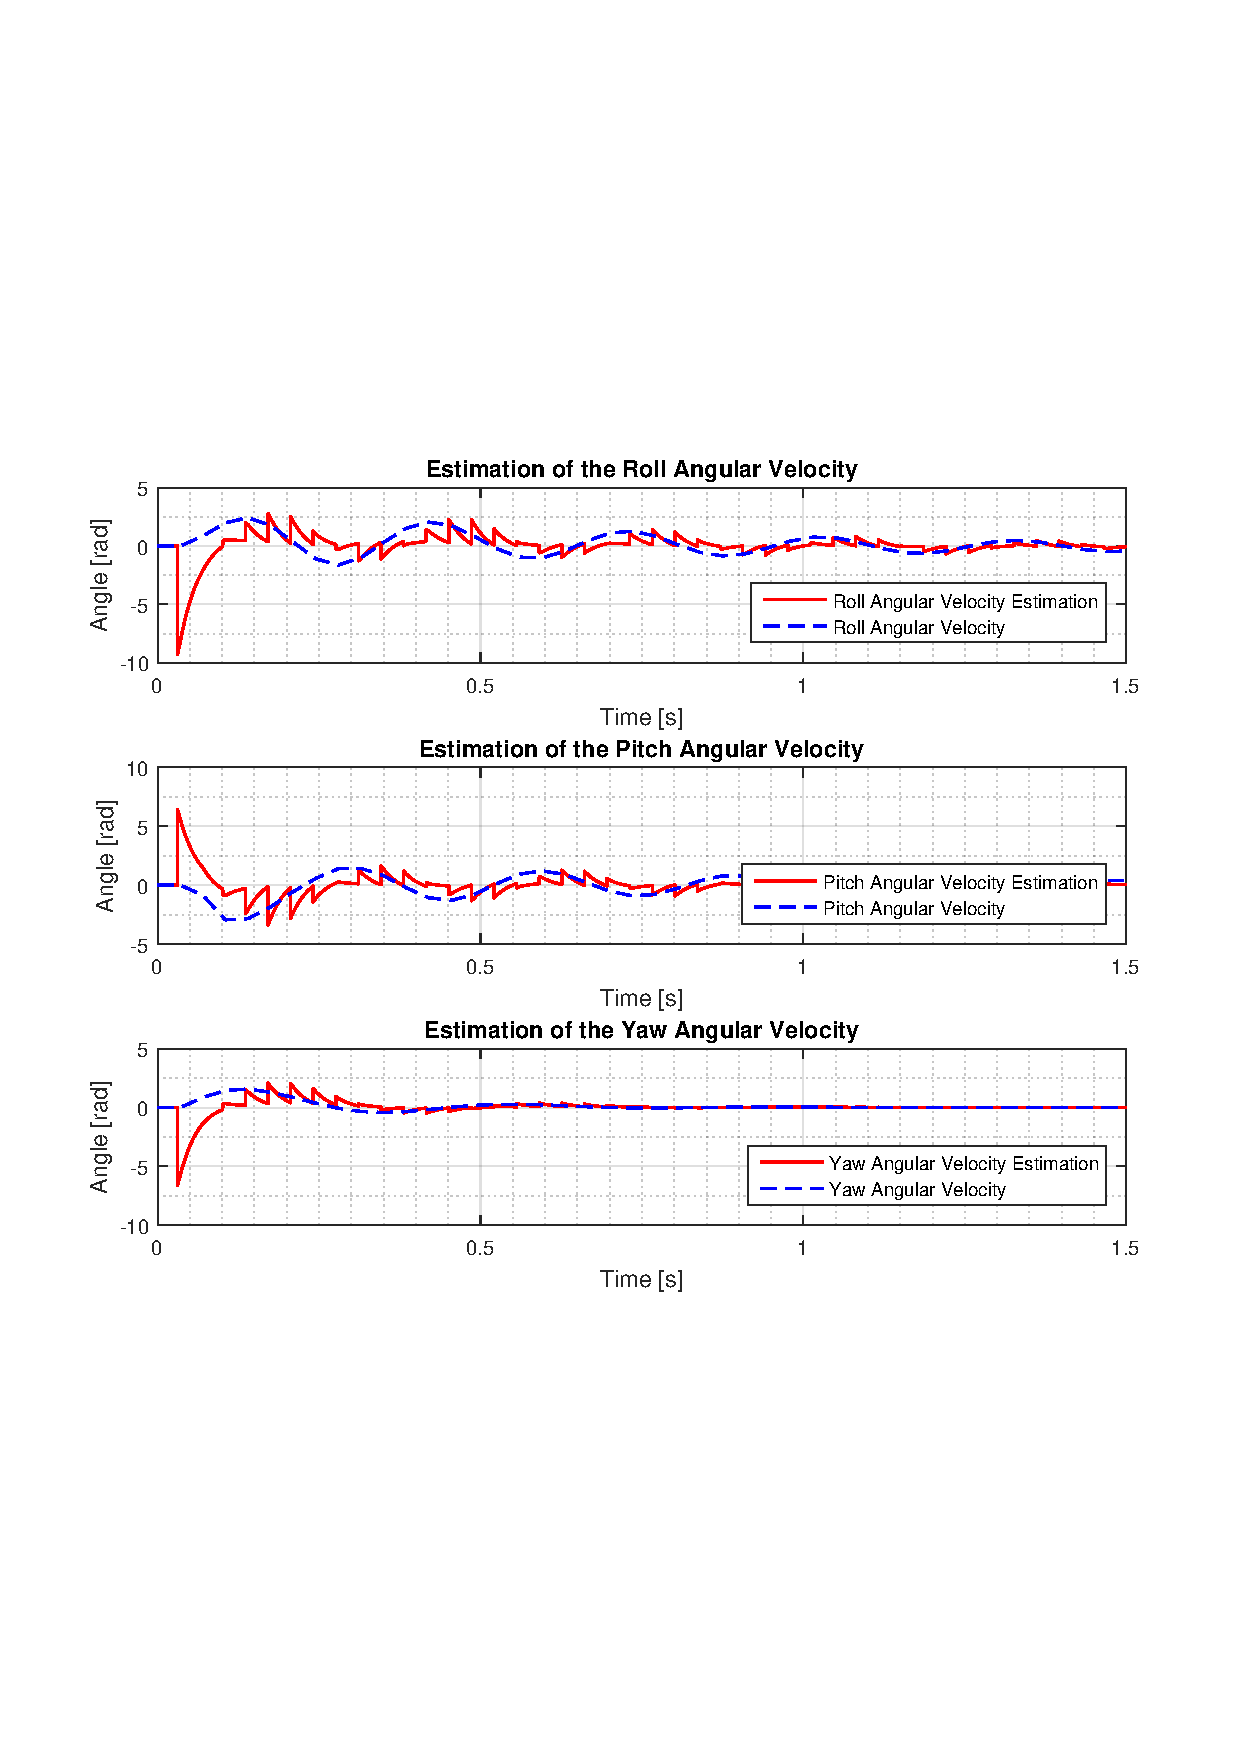
\includegraphics[scale=1]{figures/ssObsHigh.pdf}
	\caption{\autoref{app:matricesSS}.}
	\label{fig:TranslationalControlDiagram}
\end{figure}

\begin{figure}[H]
	\centering
	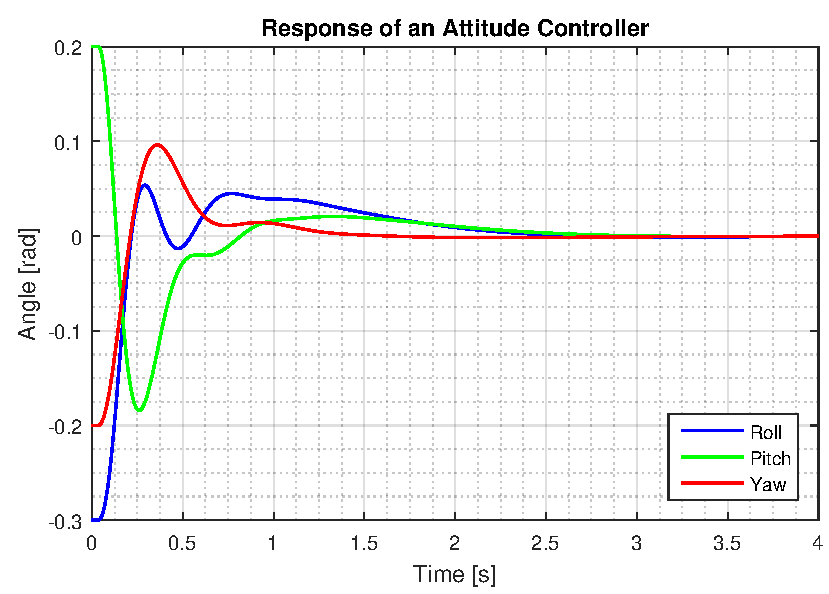
\includegraphics[scale=1]{figures/ssEqObsFinal.pdf}
	\caption{\autoref{app:matricesSS}.}
	\label{fig:TranslationalControlDiagram}
\end{figure}

\begin{figure}[H]
	\centering
	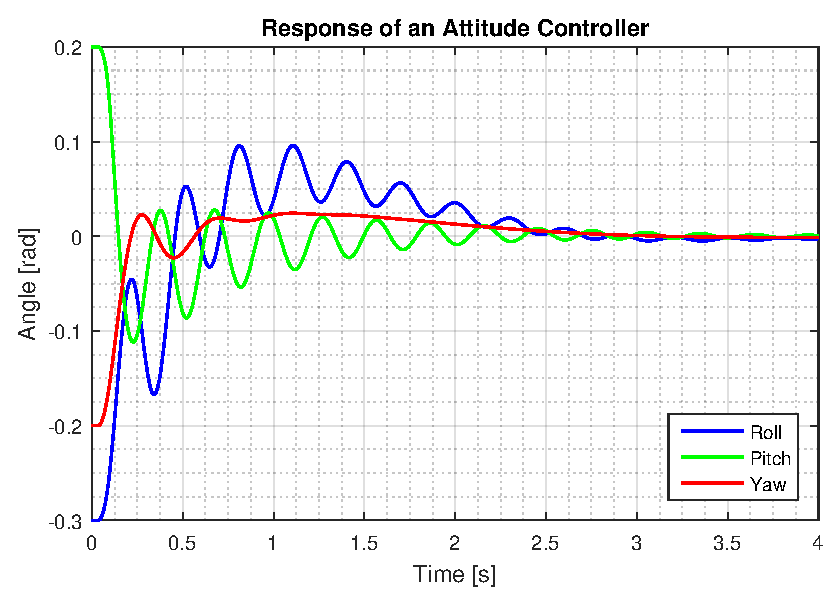
\includegraphics[scale=1]{figures/ssEqObsHigh.pdf}
	\caption{\autoref{app:matricesSS}.}
	\label{fig:TranslationalControlDiagram}
\end{figure}
